
\begin{frame}[fragile]{Yocto Image}
	\begin{multicols}{2}
		\begin{lstlisting}[title=mume-dev-image.bb,frame=single,language=bitbake]
LICENSE = "MIT"

inherit core-image
inherit populate_sdk_qt5

IMAGE_INSTALL = " \
  packagegroup-core-boot \
  @\ldots@-core-ssh-openssh \
  packagegroup-mume-common \
  packagegroup-dev-mume \
"

IMAGE_FEATURES += " \
  package-management \
  debug-tweaks \
"
		\end{lstlisting}
		\begin{lstlisting}[title=packagegroup-dev-mume.bb, frame=single, numbers=right, language=bitbake]
SUMMARY = "developer tools for MUME"
LICENSE = "MIT"

inherit packagegroup

RDEPENDS_${PN} = "\
  bash \
  devmem2 \
  htop \
  nginx \
  openssh-sftp \
  perf \
  qtbase \
  time \
  @\ldots@
		\end{lstlisting}
	\end{multicols}
\end{frame}

\begin{frame}[fragile]{Yocto Image bauen}
	\begin{lstlisting}[frame=single,language=bash, basicstyle=\small\ttfamily]
$ bitbake mume-dev-image
	\end{lstlisting}
	\begin{table}
		\caption{tmp/deploy/images/beaglebone/}
		\begin{tabular}{ll}
			\hline MLO & stage 1 loader \\ 
			\hline u-boot.img & stage 2 loader \\ 
			\hline uEnv.txt & u-boot Konfiguration \\ 
			\hline zImage & Kernel \\ 
			\hline zImage-bonegreen-mume.dtb & Device Tree \\ 
			\hline mume-dev-image-beaglebone.tar.bz2 & rootfs \\ 
			\hline 
		\end{tabular} 
	\end{table}
\end{frame}

\begin{frame}[fragile]{rootfs}
	\begin{lstlisting}[frame=,numbers=none,escapeinside={@}{@},language=,basicstyle=\small\ttfamily]
/
  bin
  boot
  etc
  home
  lib
  mnt
  opt
  root
  tmp
  usr
  var
  @\ldots@
	\end{lstlisting}
	\only<handout>{
		\begin{itemize}
			\item userspace
			\item ev. Kernel \& Device Tree
			\item nicht bootloader
		\end{itemize}
	}
\end{frame}

\begin{frame}[fragile]{Device Tree}
	\begin{lstlisting}[frame=,numbers=none,escapeinside={|}{|},language=,basicstyle=\small\ttfamily]
/ {
  compatible = "ti,am33xx";

  spi0: spi@48030000 {
    compatible = "ti,omap4-mcspi"|\hnote{Mapping zu Treiber}|;
    status = "disabled"|\hnote{aktivieren durch status="okay"}|;
    reg = <0x48030000 0x400>|\hnote{Register-Position, siehe Datenblatt des SOC}|;
    interrupts = <65>;
    dmas = <&edma|\hnote{Referenz zum DMA Device-Tree Knoten}| 16 &edma 17>;
    |\dots|
  };
|\dots|
	\end{lstlisting}
\end{frame}
\note{
	\begin{itemize}
		\item Linux kennt Hardware nicht
		\item Device Tree beschreibt Hardware
		\item Linux lädt Treiber anhand Device Tree
	\end{itemize}
}

\begin{frame}{Boot Process\hcite{OMAPBootloaderOverview}}
	\begin{center}
		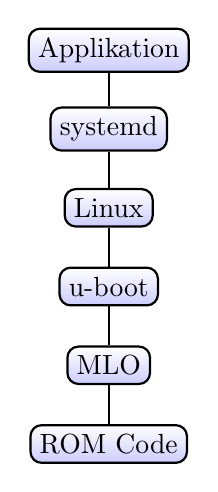
\begin{tikzpicture}[thick]
			\tikzstyle{every node}=[shape=rectangle, rounded corners,
				draw, align=center, top color=white, bottom color=blue!20]

			\visible<2->{
				\node at (0,0) (rom) {ROM Code};
			}

			\visible<3->{
				\node at (0,1) (mlo) {MLO};
				\draw (rom) -- (mlo);
			}

			\visible<4->{
				\node at (0,2) (uboot) {u-boot};
				\draw (mlo) -- (uboot);
			}

			\visible<5->{
				\node at (0,3) (linux) {Linux};
				\draw (uboot) -- (linux);
			}

			\visible<6->{
				\node at (0,4) (systemd) {systemd};
				\draw (linux) -- (systemd);
			}

			\visible<7->{
				\node at (0,5) (app) {Applikation};
				\draw (systemd) -- (app);
			}
		\end{tikzpicture}
	\end{center}\end{frame}
\note{
	\scriptsize{
		\begin{tabular}{|l|l|l|}
			\hline Typ & Name & Funktion \\ 
			\hline System startup & ROM Code & minimale Hardware Initialisierung \\ 
			& & in Boot-Devices nach Stage 1 Loader suchen \\
			& & Stage 1 Loader ins RAM laden und ausführen \\
			
			\hline Stage 1 Loader & MLO & Pin Muxing \\ 
			& x-loader & Clock und Memory initialisieren \\
			& (u-boot) & Stage 2 Loader ins RAM laden und ausführen \\
			
			\hline Stage 2 Loader & u-boot.img & Plattform Initialisierung (USB, Netzwerk, \ldots) \\
			& & Boot-Menü / Kommandozeile anzeigen \\
			& & Kernel und Device-Tree ins RAM laden und ausführen \\
			
			\hline Kernel & zImage & Treiber für Hardware laden \\ 
			& Linux & rootfs mounten \\
			& & Init-Process starten \\
			
			\hline Init & Systemd & Abhängigkeiten zwischen Services auflösen \\ 
			& & Services starten \\
			& & Services überwachen \\
			
			\hline 
		\end{tabular} 
	}
}

\begin{frame}[fragile]{SDK bauen}
	\pause
	\begin{lstlisting}[frame=single,language=bash, breaklines=true, basicstyle=\small\ttfamily]
$ bitbake mume-dev-image -c populate_sdk
$ ls -sh tmp/deploy/sdk/
695M mume-glibc-x86_64-mume-dev-image-cortexa8hf-vfp-neon-toolchain-2.0.sh
	\end{lstlisting}
	\pause
	\begin{itemize}
		\item Cross-Compiler
		\item rootfs (Libraries, \ldots)
		\item Entwicklerpakete (Header, \ldots)
		\item Paketmanager
	\end{itemize}
\end{frame}
